\section{Daniel Wagner}
\textbf{Responsibility: Scale sourcing, experimental scale integration, web-app frontend and  backend}\\
\textbf{Role: Communication Master}\\

\subsection{Scale sourcing}

To develop a proof of concept it was required to show 3rd party medical devices could be integrated into our system. For this purpose, we decided to use either blood pressure measurement devices or body analysis scales. The reason for choosing those device categories is that relatively speaking they are simpler to integrate into a project that is supposed to be built upon none proprietary hardware, firmware and software while at the same time still having the capability to capture relevant medical data for our use case [1.2]. We further narrowed down our scope of relevant devices by conversing with our project owner and medical professional Tobias Steigleder. We then screened Opensource code platforms and forums for code that would allow us to integrate some of these devices. Based on the ability to be integrated into our project and other criteria like price, market availability and quality of measurements the following devices made it into our closer selection:

Respiratory Rate / Blood pressure:

\begin{itemize}
	\item Soehnle Blood Pressure Monitor Systo Monitor Connect 300

	\item Omron RS7 Intelli IT Wrist Blood Pressure Monitor

	\item Beurer BM 54 Bluetooth Blood Pressure Monitor
\end{itemize}

Weight/ Body composition:

\begin{itemize}
	\item Kamtron Bluetooth Digital Personal Scales

	\item Vigorun Smart Bluetooth Electronic Body Fat Scales

	\item Beurer BF 700 Diagnostic Bathroom Scales\\

\end{itemize}

Subsequently tests in a local technology store could be performed to further assess the viability of the devices pre-purchase. However not just the devices above were tested but the whole sortiment of the Mediamarkt and Expert stores. The tests were performed by using the Nordic Semiconductor nRF Connect app as well as the development version of the Openscale app\footnote{https://github.com/oliexdev/openScale}. The tests were performed with phones that used different physical layers (phy1M and phy2M) as this can have an impact on the signals that are being received on the host device. This knowledge is based on previous experience with the ESP32 microcontroller and experiments with different android phones. Other factors to consider are turning on location services on the phones when trying to connect to a Bluetooth Low Energy (=BLE) device. It is recommended to install the manufacturers app to establish the first connection to the BLE server device (scale). After connecting for the first time the manufacturer apps should be closed as they can interfere with the debugging apps and the phone system as they usually are very unstable or do not work at all on some devices. Debugging the BLE connection which involved reading out characteristics and services with the nRF Connect app became possible for most scales that supported BLE. Testing scales with the openscale project was only feasible for scales that were supported. 

In the end the Beurer BF700 was chosen for the following reasons:

\begin{itemize}
	\item internal measurement cache with support for different profiles and the ability to delete all data

	\item existing documentation and support in Open Scale project as well as positive comments on the project page for this particular scale

	\item 5 years warranty and good brand reputability

	\item intuitive measurement procedure for weight, fat, hydration all in one and different Bluetooth Low Energy data streams for the respective measurement

	\item one of the best manufacturer apps
\end{itemize}

\subsection{Experimental scale integration}

Gray box testing was performed on the Openscale code to understand its functionality, find potential bugs and identify the pieces that could be used for our own project. First the whole app was segmented, analyzed and sequentially stripped from the modules that were not essential to realizing a BLE connection and receiving data. This turned out to be difficult as the author very tightly coupled data management and BLE connection handling. The following mindmap shows the structure of the Openscale project, what components were used for the production build (orange) and for the development build (purple). All other components were ditched with the aim to create a lean app that with as few conflicts as possible with code that we wrote and Openscale code.

\begin{figure}[h]
	\centering
	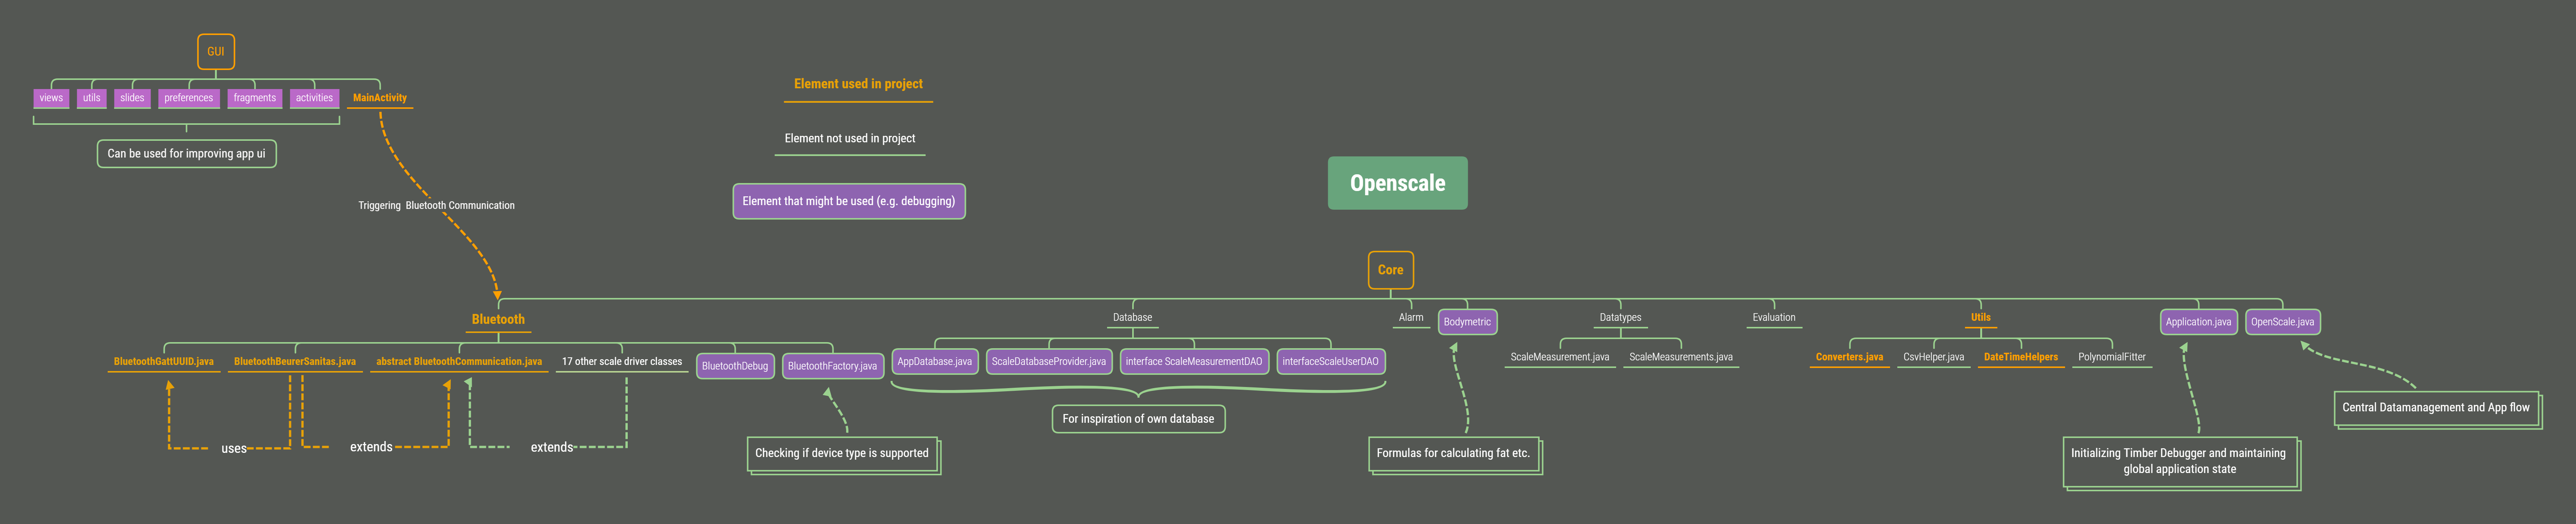
\includegraphics[width=\textwidth,height=2.0in]{./media/image1.png}
	\caption{Openscale project overview}
\end{figure}

\subsection{Setup of web-app project}

Our web project consisted of two parts. The backend should aggregate data from the patient ‘s phone app as well as relay this data back to any frontend that would display it. A few system design decisions were made for realizing this. The backend framework we used was Django which suited itsself to our team as some members had previous experience with it and it quickly allows you to get started. Other reasons for choosing Django include that there is an active developer community, the fact that it is a well-maintained project and that there is a plethora of documentation available.

For the frontend React JS was chosen for mostly the same reasons as Django. Both work nicely together and there exist many projects that use the two technologies in tandem. The fundamental idea of the software stack is that Django would serve static files on a webserver. This included images, html, css and most importantly the compiled React Javascript code. Although not splitting frontend and backend into two seperate code bases might not be very common in software development, this allowed us to package the web-app more tightly. This also made a faster development workflow and fully leveraging Django ‘s capabilities possible.

Django ‘s functionality can be explained with the Model View Controller concept\footnote{https://djangobook.com/mdj2-django-structure/}. Essentially when a URL is called in the browser a method of a view object is triggered. The view can then make database calls via model objects and start executing code on the server. In our project we used views to perform authentication, load frontend code as well as loading and saving data to and from the backend.

\begin{figure}[h]
	\advance
	\leftskip 0.05in	
	\centering
	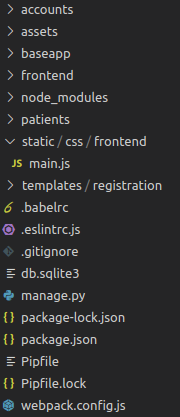
\includegraphics[width=1.87in,height=4.34in]{./media/image2.png} \caption{Web project folder structure}

\end{figure}

In Django different apps can be created to seperate functionality within the entire web app. Each app can define its own URLs that trigger the respective view method as well as the models that manage database functionality. The accounts app was used to expose an API for authentication. Assets stored image or animation files. Baseapp is the entry point for the entire project and is used to configure libraries, the behaviour and priority in which other Django apps are loaded as well as telling Django where certain files are located. Frontend is a placeholder app whose purpose it is to load the compiled React code. Patients manages all patient data and offers it in form of a REST API. Manage.py is the shell console with which all the Django server can be controlled. All other folders and files are used for frontend purposes. Node\_modules stores all React library modules. Static / css / frontend stores all compiled Javascript code that Django can serve via its frontend app. In templates html files (e.g. login forms) can be stored. .babelrc is the configuration file for Babel which is a compiler and syntax transformer for Javascript. It's main usage is to use newer syntax without waiting for browser support as the the compiled javascript becomes backwards compatible. package.json defines all libraries that should be loaded with Javascript package managers like npm. Pipfile defines all the python packages that should be loaded for Django. For this to work pipenv should be installed on the system. Lastly webpack.config.js is the config file for Webpack which compiles and bundles all frontend source code into one single file that Django can load and render websites with. 

\subsection{Backend development}

When a URL is called that points to the IP of the webserver the first thing that happens is that Django starts searching for a route in the ‘baseapp’ app urls.py file. First it checks whether the admin panel was called (127.0.0.1:8000/admin/). If this is not the case API calls for the patient REST API (127.0.0.1:8000/patients) or accounts authentication API (127.0.0.1:8000/auth) are handled first. Only after those are handled, Django will try to render the frontend (127.0.0.1:8000). This distinction is important so that Django does not try to handle API calls when no route is entered. \\

\textbf{Patients API}

This API was realized via the Django Rest Framework whose general functionality was described before (4.4). More specifically the ‘patients’ app defines all database fields that are managed in the models.py file. These fields are then converted to JSON with the serializers.py file. The api.py file then takes that JSON data and exposes all of it to the API endpoint (127.0.0.1:8000/patients).

When calling the API URL all patient data like midos status or health status can be accessed in one JSON object. \\

\begin{lstlisting}[label={lst:mylabel}, caption={'Patients' JSON object},captionpos=b, basicstyle=\small, tabsize=3]
	[
		{
			"id": 2,
			"first_name": "Adriana",
			"last_name": "C. Ocampo Uria",
			"last_update": "2019-12-21T15:18:26.666167Z",
			"midos_status": "good",
			"health_status": "medium"
		}, 
		{
			"id": 3,
			"first_name": "Edmond",
			"last_name": "Halley",
			"last_update": "2019-12-21T15:18:45.070093Z",
			"midos_status": "bad",
			"health_status": "medium"
		},
		{
			"id": 4,
			"first_name": "Gertrude",
			"last_name": "B. Elion",
			"last_update": "2019-12-21T15:18:55.977195Z",
			"midos_status": "critical",
			"health_status": "critical"
		},
		...
	]
\end{lstlisting}


\textbf{Authentication}

JSON Web Tokens\footnote{https://jwt.io/} (=JWT) were used for authentication and protection of the API endpoints. The ‘patients’ API can only be accessed when a token authentication has been performed. This is handled with three URLs: 127.0.0.1/auth/, 127.0.0.1/refresh/, 127.0.0.1/verify/. A token can be fetched by providing login credentials to the auth URL. Its expiration time is set to 5 minutes. The token needs to be refreshed in that interval. If this does not happen the API points cannot be accessed anymore. After refreshing, a new token is generated which can then be used to refresh again. Currently this authentication system is only used for the web-app. The biggest benefit of using JWT is however, that single-sign-on systems can be realized with it. Once a user is logged out or signed in this will be the case on all devices. This can be coupled with activity tracking (e.g. tracking whether a user clicks on buttons or moves mouse) on the device being used in the moment to create a very secure system and to keep the medical data of the patients protected. Having an activity tracking system that performs auto logouts alone does not secure the API endpoints. Therefore, a server-side authentication system is required. 

\subsection{Frontend development}

\textbf{Components}

\begin{figure}[h]
 	\centering
 	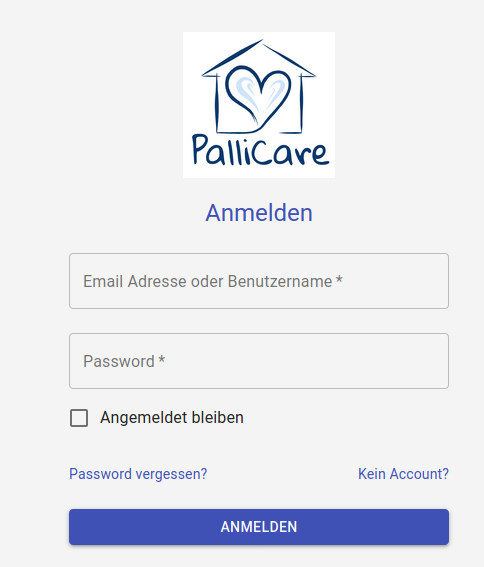
\includegraphics[width=2.65in,height=3.1in]{./media/image4.png}
 	\caption{Login screen}
\end{figure}


\begin{figure}[h]
	\centering
	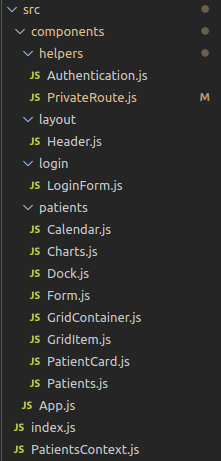
\includegraphics[width=1.7in,height=3.19in]{./media/image3.png}
	\caption{Component overview}
\end{figure}

One of React‘s most important features is its components system. Almost every function or part of the user interface will be handled by a react component. Components can have parents and children. This results in a component tree with components stacked in each other. The login screen of the app contains components that pass along information to a global context (username, password etc.). Within these components other components are nested like the image component for the logo, form components for the username and password as well as control components for the button.

On the mainscreen of the app cards were built using the material design library\footnote{https://material-ui.com/}. With the grid system\footnote{https://material-ui.com/components/grid/} the cards can be layed out and sized as wished. A grid container component containes grid item components that each contain a patient card component. Within the patient card component the midos and biometric status of the patient is translated into the words „good$``$, „medium$``$, „bad$``$ or $``$not determined$"$  and the colors green, yellow, red or gray. This data for the patients is retrieved from the ‘PatientsContext’ component. The purpose of this global context component is to provide the patients data to all its child components. ‘PatientsContext’ consumes the ‘patients’ REST api with and converts the received JSON data into javascript objects that can then be passed along down the component tree. \\

\begin{figure}[h]
  \begin{center}
    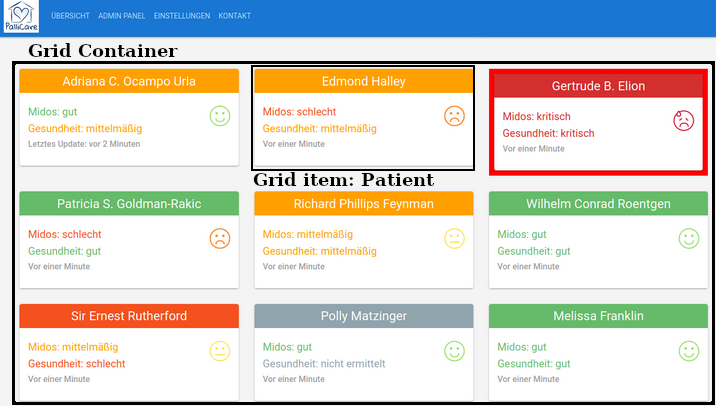
\includegraphics[width=6.17in,height=3.5in]{./media/image5.png}
  \end{center}
  \caption{Grid components}
  \label{fig:helptext2}
\end{figure} 

\textbf{Dock}

To see more details about one specific patient a dock\footnote{https://www.npmjs.com/package/react-dock} was implemented. On the click of a button it folds out and covers a large part of the screen. The dock can be closed with a button to the top left. Because the frontend was inspired by single page web-apps where one single source of information fuels all functionality this dock also uses the data of ‘patients’ context. It can be used to display graphs for example. A calendar will in the future allow a date range to be selected in which to view the patient data. \\

\begin{figure}[h]
	\centering
	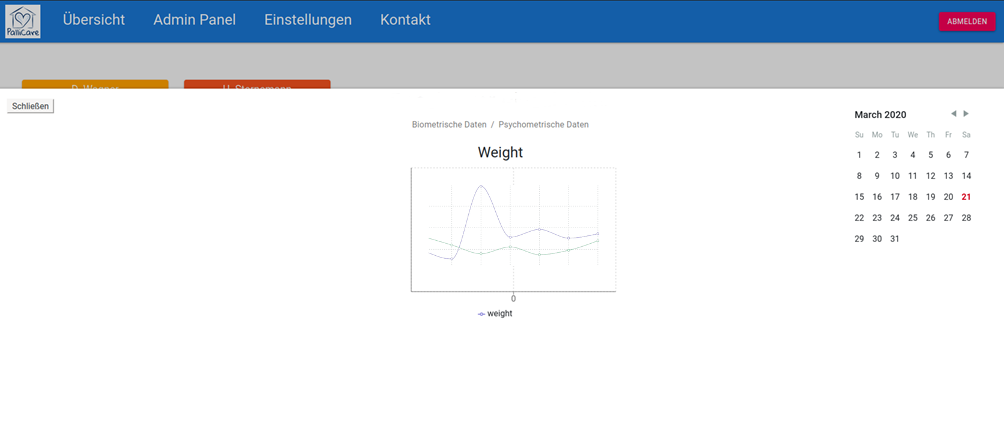
\includegraphics[width=6.69in,height=2.93in]{./media/image6.png}
	\caption{Expanded dock}
\end{figure}


\textbf{Security}

For realizing the auto logout feature of the web-app JWT, activity tracking\footnote{https://www.npmjs.com/package/react-idle-timer} and private routes\footnote{https://reacttraining.com/react-router} were leveraged. JWT tokens are getting obtained, refreshed and verified as soon as the user logs in and is active. Being active is determined by the user triggering mouse events like a button click or mouse movement. Should the user not be active for 10 minutes an auto logout will be performed and the JWT token will no longer be refreshed. This was done using a public route to the login screen and a private route that can only be accessed after user typed in the right credentials and if the JWT token is alive as well as if the user is active. To store the authentication status and perform the JWT verification for example a global context class like in PatientsContext.js was used in Authentication.js. 
